\documentclass[10pt,a4paper]{beamer}
\usepackage[latin1]{inputenc}
\usepackage{amsmath}
\usepackage{amsfonts}
\usepackage{amssymb}
\usepackage{graphicx}
\usetheme{PaloAlto}
\logo{\colorbox{white}{
\includegraphics[scale=0.5]{aau_logo_new_circle}}} 


\begin{document}

	\title{sw608f14 - Piktotegner}
	\author{Daniel S. F, Lars A, Mathias W. P. \& S�ren S. A.}
	
	
	\begin{frame}[plain,noframenumbering]
	\titlepage
	\end{frame}
	
	
	\section{Multi Project}
	\begin{frame}
	\frametitle{Multi Project}
		\begin{itemize}
		\item GIRAF
		\item Large Setting
		\item SCRUM
		\item Tools
		\item Specialists
		\end{itemize}
		More slides may be added for each item here.
	\end{frame}
	
	
	\section{Old Piktotegner}
		\begin{frame}
		\frametitle{Old Piktotegner}
		\begin{figure}
			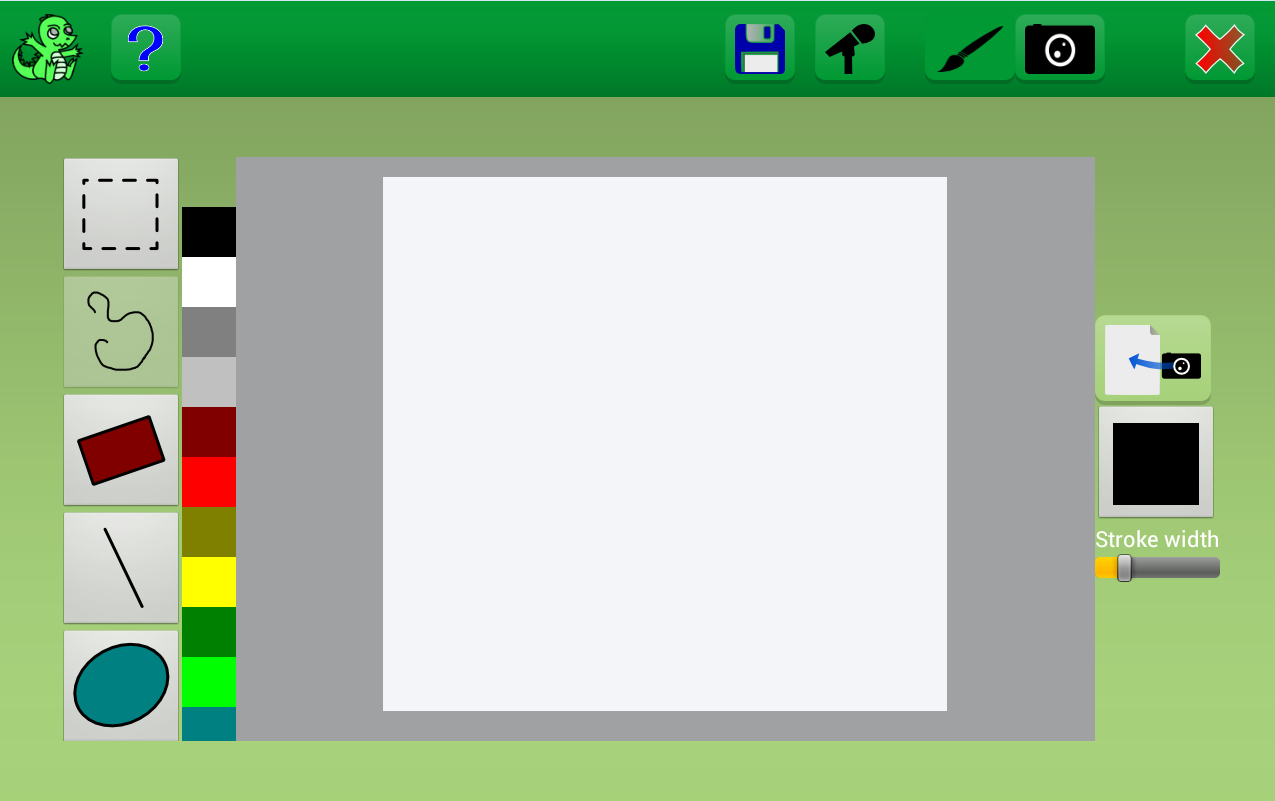
\includegraphics[width=\textwidth]{media/CrocOldCanvas}
			\caption{Old Piktotegner Layout}
		\end{figure}
		\end{frame}
	
	\section{Key Changes}
	\begin{frame}
	\frametitle{Key Changes}
		Each key changes listed here will have slides for that given change. Before and after pictures will be shown for this.
		\begin{itemize}
		\item Rotation
		\item Resize
		\item Collision detection
		\item Recording audio
		\item Saving and loading for piktograms
		\item Camera
		\end{itemize}
	\end{frame}
	
	\section{Usability test}
		\begin{frame}
		\frametitle{Usability test}
		\begin{itemize}
			\item Why?
			\item How?
			\item Results
		\end{itemize}
	
		\end{frame}
	
	\section{Media Library Collaboration}
		\begin{frame}
		\frametitle{Media Library Collaboration}
		\begin{itemize}
			\item MediaPlayer
			\item Text to Speech
			\item Collaboration experience
		\end{itemize}

		\end{frame}
		
	\section{Demonstration}
	\frametitle{Demonstration}
		\begin{frame}
		Here use an emulator to present the developed product, or preferably with a tablet.
			\begin{figure}
				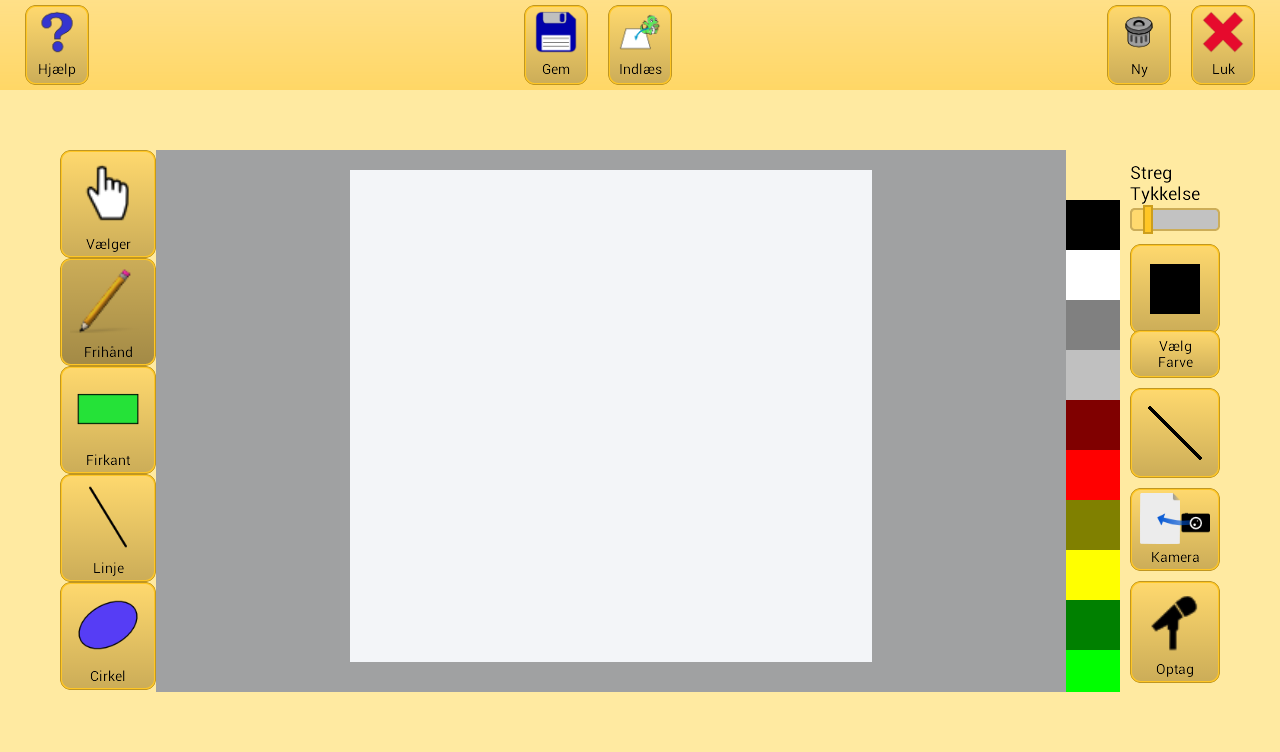
\includegraphics[width=\textwidth]{media/final-main-ui}
				\caption{New Piktotegner Layout}
			\end{figure}
		\end{frame}		

	\section{Reflections}
		\begin{frame}
		\frametitle{Reflections}
		\begin{itemize}
			\item Usability test experience gain
			\item SCRUM experience
			\item Customer interaction
			\item Further Development
		\end{itemize}
		More points to be added
		\end{frame}
	
\end{document}